% Generated by pysimcount.pffigure -- do not edit; regenerate instead.
% figure: B-all-by-formula -- Every formula at measured r
% source: results/pf-thesis/results.json
% metric=cnot gatebase=cz merged
% seed=1 t=n template=simcount synth=pygridsynth
% git_commit=04cd66abb614bdc66fb48e891cef085a299e0ab1 git_dirty=False
% source_sha256=018e0b7603e6fc9f6ee358974f241415a3b93437700847b033937cc1d4250db8
% derived: B-all-by-formula.tex with Lie-Trotter S1 removed by pysimcount.figdrop (Lie-Trotter S1 alone spans 39% of the original y-axis); removed legends: Lie-Trotter S1; source_sha256=8a1c7ef1e47f211d5155c66042c740a8767bb8a845836b2575a38730499756d9
% derived: B-all-by-formula-no-lie-trotter.tex restyled by pysimcount.figuniform: extrapolated points (r from power-law fit) drawn in their series' measured style, style-key legend entries removed; extrapolated n = [13, 20]; source_sha256=f5246deabb095668848c73ace876d3dbbce17166136abe4e6cce91298cd83b8f
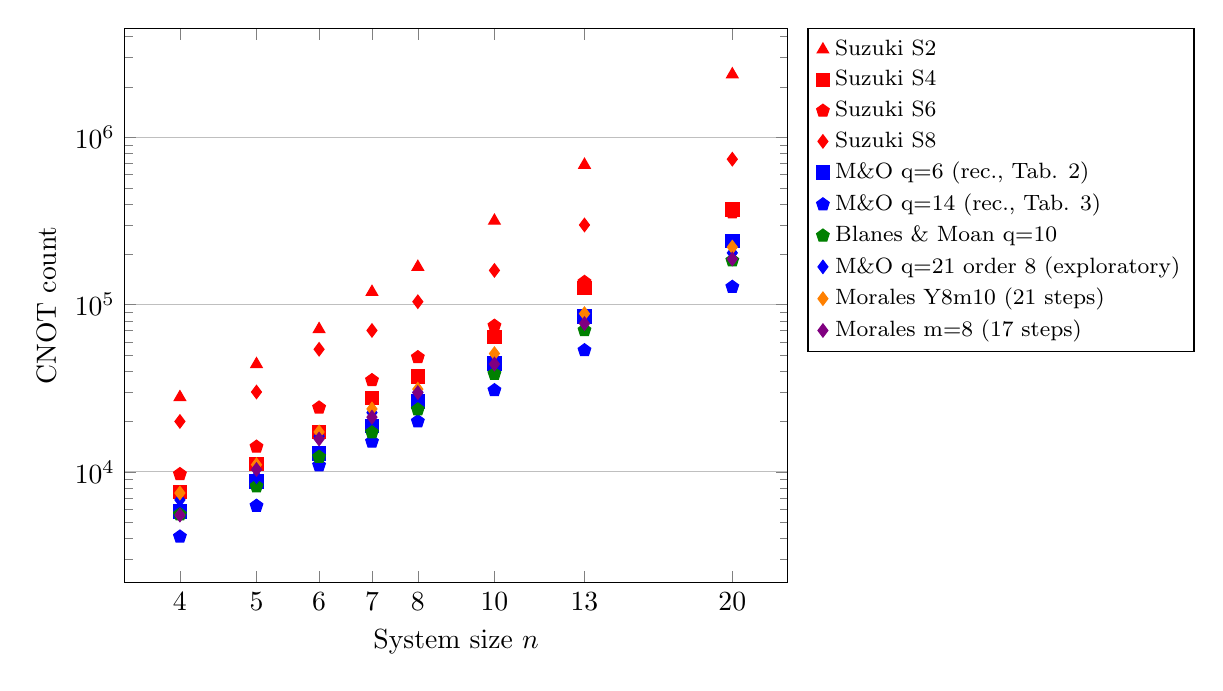
\begin{tikzpicture}
  \begin{loglogaxis}[
    width=10cm,
    xlabel={System size $n$},
    ylabel={CNOT count},
    xtick={4,5,6,7,8,10,13,20},
    xticklabels={4,5,6,7,8,10,13,20},
    ymajorgrids=true,
    legend pos=outer north east,
    legend cell align=left,
    legend style={font=\footnotesize},
  ]
    % r from power-law fit (extrapolation); one legend entry per series
    \addplot[only marks, red, mark=triangle*, mark size=2.4pt, mark options={solid, fill=red}] coordinates {
      (4,27960)
      (5,44050)
      (6,71340)
      (7,119070)
      (8,168160)
      (10,317400)
    };
    \addlegendentry{Suzuki S2}
    % r from power-law fit (extrapolation); one legend entry per series
    \addplot[only marks, red, mark=triangle*, mark size=2.4pt, mark options={solid, fill=red}, forget plot] coordinates {
      (13,685360)
      (20,2381200)
    };
    \addplot[only marks, red, mark=square*, mark size=2.4pt, mark options={solid, fill=red}] coordinates {
      (4,7560)
      (5,11130)
      (6,17388)
      (7,27636)
      (8,37296)
      (10,63840)
    };
    \addlegendentry{Suzuki S4}
    % r from power-law fit (extrapolation); one legend entry per series
    \addplot[only marks, red, mark=square*, mark size=2.4pt, mark options={solid, fill=red}, forget plot] coordinates {
      (13,125580)
      (20,371280)
    };
    \addplot[only marks, red, mark=pentagon*, mark size=2.4pt, mark options={solid, fill=red}] coordinates {
      (4,9696)
      (5,14140)
      (6,24240)
      (7,35350)
      (8,48480)
      (10,74740)
    };
    \addlegendentry{Suzuki S6}
    % r from power-law fit (extrapolation); one legend entry per series
    \addplot[only marks, red, mark=pentagon*, mark size=2.4pt, mark options={solid, fill=red}, forget plot] coordinates {
      (13,136552)
      (20,355520)
    };
    \addplot[only marks, red, mark=diamond*, mark size=2.4pt, mark options={solid, fill=red}] coordinates {
      (4,20040)
      (5,30060)
      (6,54108)
      (7,70140)
      (8,104208)
      (10,160320)
    };
    \addlegendentry{Suzuki S8}
    % r from power-law fit (extrapolation); one legend entry per series
    \addplot[only marks, red, mark=diamond*, mark size=2.4pt, mark options={solid, fill=red}, forget plot] coordinates {
      (13,299598)
      (20,741480)
    };
    \addplot[only marks, blue, mark=square*, mark size=2.4pt, mark options={solid, fill=blue}] coordinates {
      (4,5800)
      (5,8750)
      (6,12900)
      (7,18900)
      (8,26400)
      (10,44500)
    };
    \addlegendentry{M\&O q=6 (rec., Tab. 2)}
    % r from power-law fit (extrapolation); one legend entry per series
    \addplot[only marks, blue, mark=square*, mark size=2.4pt, mark options={solid, fill=blue}, forget plot] coordinates {
      (13,85150)
      (20,241000)
    };
    \addplot[only marks, blue, mark=pentagon*, mark size=2.4pt, mark options={solid, fill=blue}] coordinates {
      (4,4104)
      (5,6270)
      (6,10944)
      (7,15162)
      (8,20064)
      (10,30780)
    };
    \addlegendentry{M\&O q=14 (rec., Tab. 3)}
    % r from power-law fit (extrapolation); one legend entry per series
    \addplot[only marks, blue, mark=pentagon*, mark size=2.4pt, mark options={solid, fill=blue}, forget plot] coordinates {
      (13,53352)
      (20,127680)
    };
    \addplot[only marks, green!50!black, mark=pentagon*, mark size=2.4pt, mark options={solid, fill=green!50!black}] coordinates {
      (4,5576)
      (5,8200)
      (6,12300)
      (7,17220)
      (8,23616)
      (10,38540)
    };
    \addlegendentry{Blanes \& Moan q=10}
    % r from power-law fit (extrapolation); one legend entry per series
    \addplot[only marks, green!50!black, mark=pentagon*, mark size=2.4pt, mark options={solid, fill=green!50!black}, forget plot] coordinates {
      (13,70356)
      (20,183680)
    };
    \addplot[only marks, blue, mark=diamond*, mark size=2.4pt, mark options={solid, fill=blue}] coordinates {
      (4,6800)
      (5,9350)
      (6,16320)
      (7,22610)
      (8,29920)
      (10,47600)
    };
    \addlegendentry{M\&O q=21 order 8 (exploratory)}
    % r from power-law fit (extrapolation); one legend entry per series
    \addplot[only marks, blue, mark=diamond*, mark size=2.4pt, mark options={solid, fill=blue}, forget plot] coordinates {
      (13,83980)
      (20,204000)
    };
    \addplot[only marks, orange, mark=diamond*, mark size=2.4pt, mark options={solid, fill=orange}] coordinates {
      (4,7480)
      (5,11050)
      (6,17340)
      (7,23800)
      (8,31280)
      (10,51000)
    };
    \addlegendentry{Morales Y8m10 (21 steps)}
    % r from power-law fit (extrapolation); one legend entry per series
    \addplot[only marks, orange, mark=diamond*, mark size=2.4pt, mark options={solid, fill=orange}, forget plot] coordinates {
      (13,88400)
      (20,221000)
    };
    \addplot[only marks, violet, mark=diamond*, mark size=2.4pt, mark options={solid, fill=violet}] coordinates {
      (4,5520)
      (5,10350)
      (6,15732)
      (7,21252)
      (8,29808)
      (10,44160)
    };
    \addlegendentry{Morales m=8 (17 steps)}
    % r from power-law fit (extrapolation); one legend entry per series
    \addplot[only marks, violet, mark=diamond*, mark size=2.4pt, mark options={solid, fill=violet}, forget plot] coordinates {
      (13,77142)
      (20,187680)
    };
  \end{loglogaxis}
\end{tikzpicture}
